%! TEX root = ../main.tex
% ==============================================================
% IMMUTABLE — generated automatically, do not edit this block
%
% — Provenance ───────────────────────────────────────────────────
%   script            : plotter.py::plot_frequency_spectrum
%   computed_in       : 
%   plot_type         : spectrum_fft
%   data_class        : 
%   generated_at      : 2026-04-22T19:45:59
%   findings_doc      : 
%
% — Thesis context ──────────────────────────────────────────────
%   chapter           : 04
%   caption_label     : fig:ch04_fft_wave
%   caption_short     : FFT amplitude spectrum of the free surface during wave runs (paddle frequency 1.3\,Hz, amplitude 0.2\,V, full panel)
%
% — Filters ────────────────────────────────────────────────────
%   panel             : full
%   wind              : 
%   amplitude [V]     : 0.2
%   frequency [Hz]    : 1.3
%   probes            : 9373/170, 12400/250, 9373/340, 8804/250
%   run_category      : standard
%   quality_flag      : 
%   mooring           : 
%
% — Data provenance ────────────────────────────────────────────
%   n_runs            : 19
%   in_probes_used    : 9373/170+9373/340, 9373/250
%   out_probes_used   : 12400/170+12400/340, 12400/250
%   probe_configs     : march2026_better_rearranging, nov_normalt_oppsett
%   non_final_config_n: 2
%   datasets        :
%     PROCESSED-20260326-ProbePos4_31_FPV_2-tett6roof-under9Mooring-height100-lowrange
%     PROCESSED-20260327-ProbePos4_31_FPV_2-tett6roof-under9Mooring30-height100-lowrange
%   run_paths       :
%     wavedata/20251110-tett6roof-lowM-ekte580/fullpanel-fullwind-amp0200-freq1300-per15-depth580-mstop30-run1.csv
%     wavedata/20251110-tett6roof-lowM-ekte580/fullpanel-lowestwind-amp0200-freq1300-per15-depth580-mstop30-run1.csv
%     wavedata/20260307-ProbPos4_31_FPV_2-tett6roof/fullpanel-nowind-amp0200-freq1300-per40-depth580-mstop30-run1.csv
%     wavedata/20260307-ProbPos4_31_FPV_2-tett6roof/fullpanel-fullwind-amp0200-freq1300-per40-depth580-mstop90-run1.csv
%     wavedata/20260313-ProbePos4_31_FPV_2-tett6roof/fullpanel-nowind-amp0200-freq1300-per240-depth580-mstop30-run1.csv
%     wavedata/20260314-ProbePos4_31_FPV_2-tett6roof/fullpanel-fullwind-amp0200-freq1300-per240-depth580-mstop30-run1.csv
%     wavedata/20260321-ProbePos4_31_FPV_2-tett6roof-under9Mooring-height100-RENAMED/fullpanel-nowind-amp0200-freq1300-per240-depth580-mstop30-run1.csv
%     wavedata/20260323-ProbePos4_31_FPV_2-tett6roof-under9Mooring-height100/fullpanel-fullwind-amp0200-freq1300-per40-depth580-mstop30-run1.csv
%     wavedata/20260323-ProbePos4_31_FPV_2-tett6roof-under9Mooring-height100/fullpanel-fullwind-amp0200-freq1300-per40-depth580-mstop30-run2.csv
%     wavedata/20260323-ProbePos4_31_FPV_2-tett6roof-under9Mooring-height100/fullpanel-nowind-amp0200-freq1300-per40-depth580-mstop30-run1.csv
%     wavedata/20260324-ProbePos4_31_FPV_2-tett6roof-under9Mooring-height100/fullpanel-nowind-amp0200-freq1300-per240-depth580-run1.csv
%     wavedata/20260324-ProbePos4_31_FPV_2-tett6roof-under9Mooring-height100/fullpanel-fullwind-amp0200-freq1300-per40-depth580-run1.csv
%     wavedata/20260325-ProbePos4_31_FPV_2-tett6roof-under9Mooring-height100/fullpanel-nowind-amp0200-freq1300-per240-depth580-mstop30.csv
%     wavedata/20260325-ProbePos4_31_FPV_2-tett6roof-under9Mooring-height100/fullpanel-nowind-amp0200-freq1300-per240-depth580-mstop30-run1.csv
%     wavedata/20260326-ProbePos4_31_FPV_2-tett6roof-under9Mooring-height100-lowrange/fullpanel-fullwind-amp0200-freq1300-per240-depth580-mstop30-run1.csv
%     wavedata/20260327-ProbePos4_31_FPV_2-tett6roof-under9Mooring30-height100-lowrange/fullpanel-nowind-amp0200-freq1300-per240-depth580-mstop30-run1.csv
%     wavedata/20260327-ProbePos4_31_FPV_2-tett6roof-under9Mooring30-height100-lowrange/fullpanel-fullwind-amp0200-freq1300-per240-depth580-mstop30-run1.csv
%     wavedata/20260327-ProbePos4_31_FPV_2-tett6roof-under9Mooring30-height100-lowrange/fullpanel-fullwind-amp0200-freq1300-per40-depth580-mstop30-run1.csv
%     wavedata/20260327-ProbePos4_31_FPV_2-tett6roof-under9Mooring30-height100-lowrange/fullpanel-nowind-amp0200-freq1300-per40-depth580-mstop30-run1.csv
%
% — Method / numerical parameters ─────────────────────────────
%   grouper           : 
%   collapse_panels   : 
%   fft_window_hz     : 
%   extra_params      : 
%
% — Summary stats cited in caption ────────────────────────────
%   (none registered — pass extra_stats=... to build_fig_meta)
%
% — Subfigures available ───────────────────────────────────────
%     FIGURES/ch04_fft_wave.pdf
%     FIGURES/ch04_fft_wave.pdf
%     FIGURES/ch04_fft_wave.pdf
%     FIGURES/ch04_fft_wave.pdf
% ── end immutable block ─────────────────────────────────────────
\begin{figure}[htbp]
  \centering
  \begin{subfigure}[b]{0.48\linewidth}
    \centering
    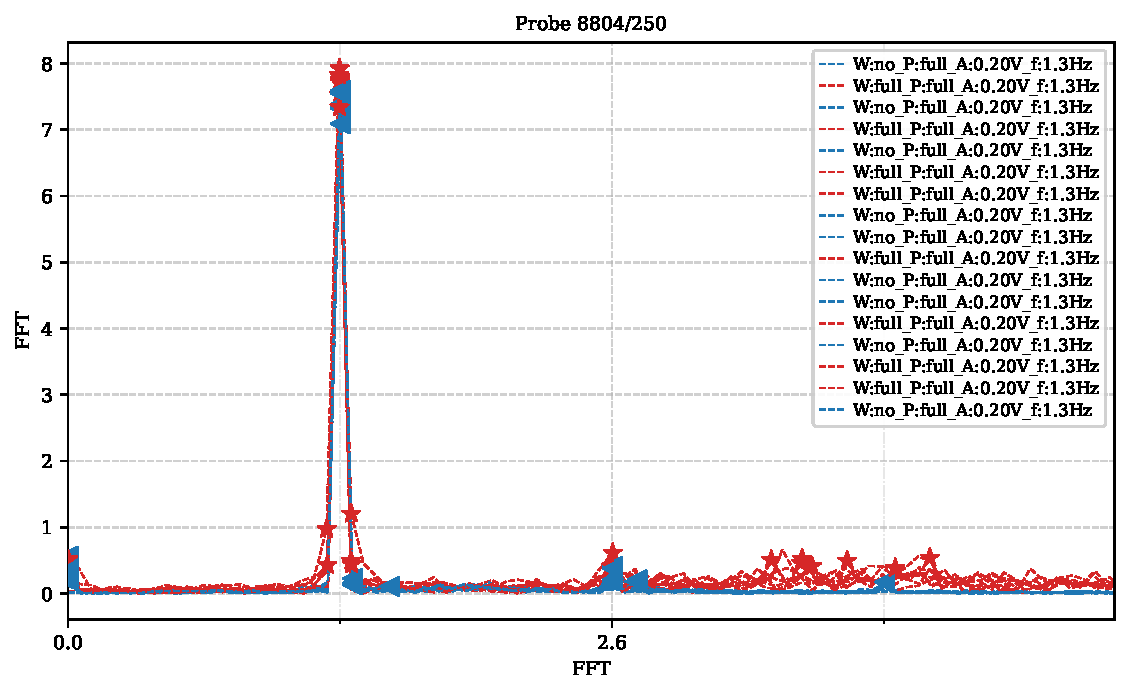
\includegraphics[width=\linewidth]{FIGURES/ch04_fft_wave.pdf}
    \caption{TODO}
    \label{fig:TODO_1}
  \end{subfigure}
  \hfill
  \begin{subfigure}[b]{0.48\linewidth}
    \centering
    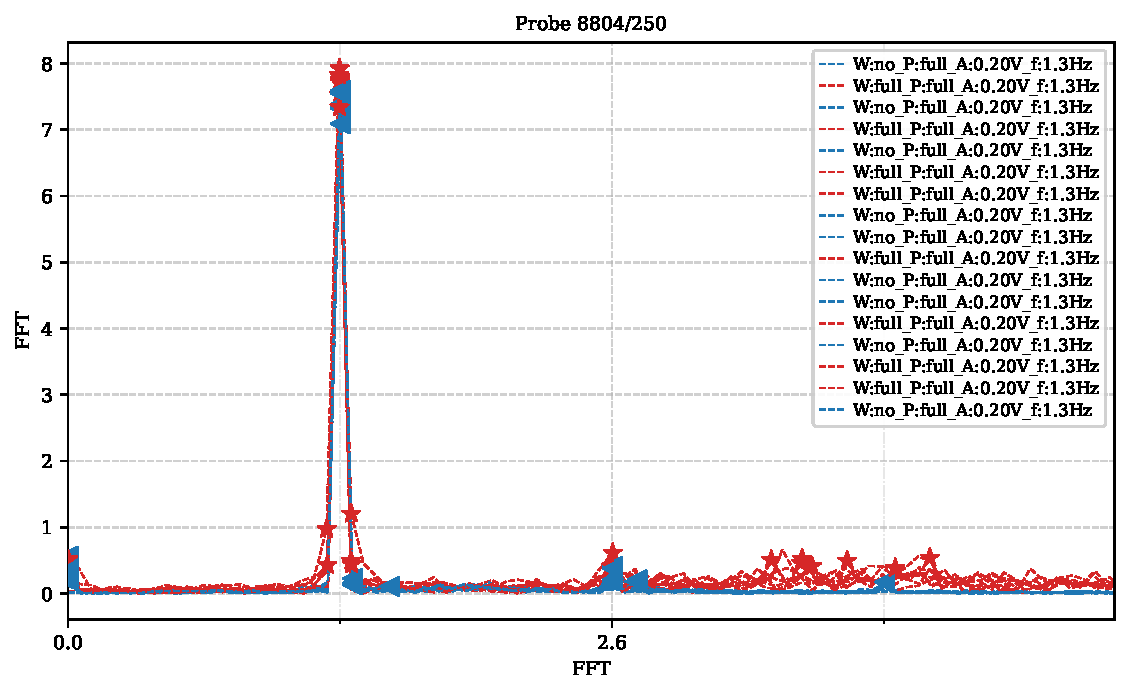
\includegraphics[width=\linewidth]{FIGURES/ch04_fft_wave.pdf}
    \caption{TODO}
    \label{fig:TODO_2}
  \end{subfigure}
  \hfill
  \begin{subfigure}[b]{0.48\linewidth}
    \centering
    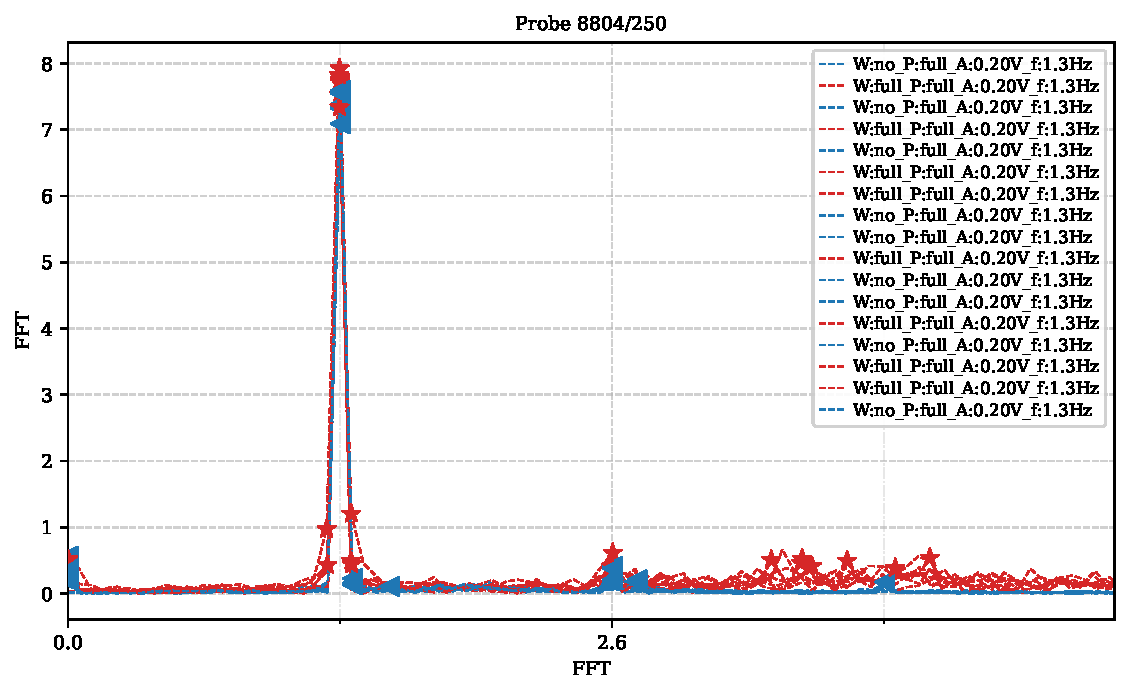
\includegraphics[width=\linewidth]{FIGURES/ch04_fft_wave.pdf}
    \caption{TODO}
    \label{fig:TODO_3}
  \end{subfigure}
  \hfill
  \begin{subfigure}[b]{0.48\linewidth}
    \centering
    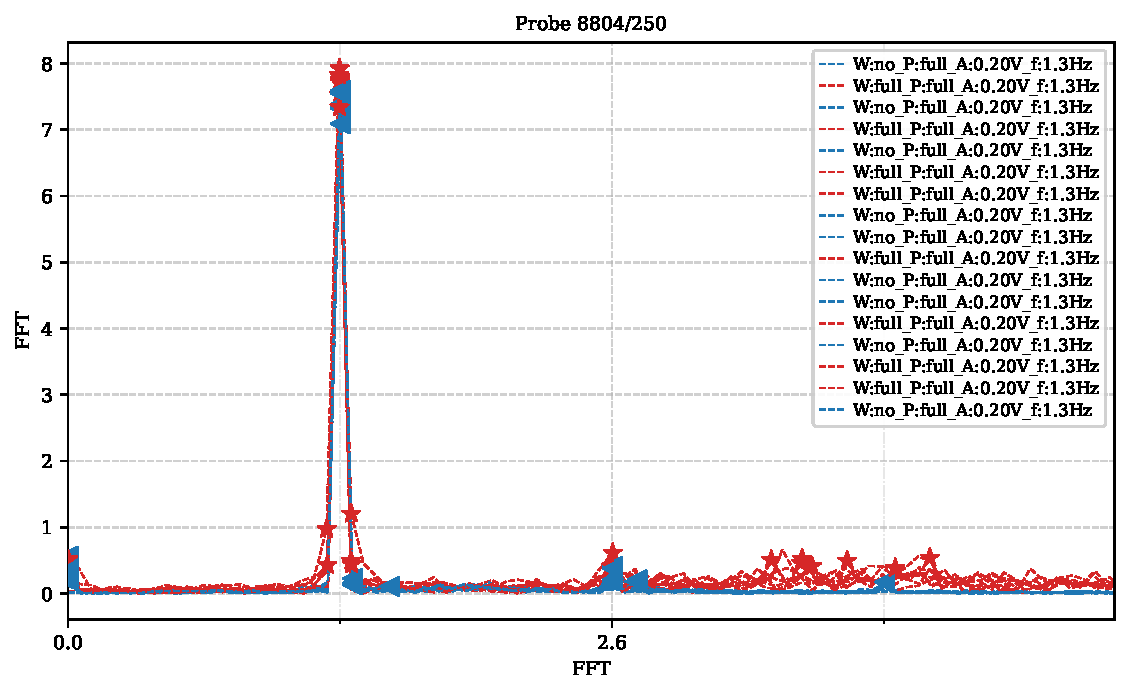
\includegraphics[width=\linewidth]{FIGURES/ch04_fft_wave.pdf}
    \caption{TODO}
    \label{fig:TODO_4}
  \end{subfigure}
  \caption[FFT amplitude spectrum of the free surface during wave runs (paddle frequency 1]{
    FFT amplitude spectrum of the free surface during wave runs (paddle frequency 1.3\,Hz, amplitude 0.2\,V, full panel). Each panel shows one probe; colour encodes wind condition. The narrow paddle-frequency peak is the target signal used for OUT/IN ratio computation.
  }
  \label{fig:ch04_fft_wave}
\end{figure}
